\documentclass{sigchi}

% Use this command to override the default ACM copyright statement
% (e.g. for preprints).  Consult the conference website for the
% camera-ready copyright statement.



%% EXAMPLE BEGIN -- HOW TO OVERRIDE THE DEFAULT COPYRIGHT STRIP -- (July 22, 2013 - Paul Baumann)
\toappear{Permission to make digital or hard copies of all or part of this work for personal or classroom use is      granted without fee provided that copies are not made or distributed for profit or commercial advantage and that copies bear this notice and the full citation on the first page. Copyrights for components of this work owned by others than ACM must be honored. Abstracting with credit is permitted. To copy otherwise, or republish, to post on servers or to redistribute to lists, requires prior specific permission and/or a fee. Request permissions from permissions@acm.org. \\
{\emph{CHI'16}}, May 07--12, 2016, San Jose, CA, USA. \\
Copyright is held by the owner/author(s). Publication rights licensed to ACM. \\
ACM 978-1-4503-3362-7/16/05 \$15.00  \\
DOI http://dx.doi.org/10.1145/2858036.2858490
}
%Copyright \copyright~2014 ACM ISBN/14/04...\$15.00. \\
%http://dx.doi.org/10.1145/2858036.2858490}
%% EXAMPLE END -- HOW TO OVERRIDE THE DEFAULT COPYRIGHT STRIP -- (July 22, 2013 - Paul Baumann)


% Arabic page numbers for submission.  Remove this line to eliminate
% page numbers for the camera ready copy 

%\pagenumbering{arabic}

% Load basic packages
\usepackage{balance}  % to better equalize the last page
\usepackage{graphics} % for EPS, load graphicx instead 
%\usepackage[T1]{fontenc}
\usepackage{txfonts}
\usepackage{times}    % comment if you want LaTeX's default font
\usepackage[pdftex]{hyperref}
% \usepackage{url}      % llt: nicely formatted URLs
\usepackage{color}
\usepackage{textcomp}
\usepackage{booktabs}
\usepackage{ccicons}
\usepackage{todonotes}
\usepackage{paralist}


% My packages
\usepackage{dcolumn}
\usepackage{multirow}
\newcolumntype{d}{D{.}{.}{4.0}}
\newcolumntype{s}{D{.}{.}{1.4}}
\usepackage{arydshln}
\usepackage{enumitem}


% llt: Define a global style for URLs, rather that the default one
\makeatletter
\def\url@leostyle{%
  \@ifundefined{selectfont}{\def\UrlFont{\sf}}{\def\UrlFont{\small\bf\ttfamily}}}
\makeatother
\urlstyle{leo}

% To make various LaTeX processors do the right thing with page size.
\def\pprw{8.5in}
\def\pprh{11in}
\special{papersize=\pprw,\pprh}
\setlength{\paperwidth}{\pprw}
\setlength{\paperheight}{\pprh}
\setlength{\pdfpagewidth}{\pprw}
\setlength{\pdfpageheight}{\pprh}

% Make sure hyperref comes last of your loaded packages, to give it a
% fighting chance of not being over-written, since its job is to
% redefine many LaTeX commands.
\definecolor{linkColor}{RGB}{6,125,233}
\hypersetup{%
  pdftitle={SIGCHI Conference Proceedings Format},
  pdfauthor={LaTeX},
  pdfkeywords={SIGCHI, proceedings, archival format},
  bookmarksnumbered,
  pdfstartview={FitH},
  colorlinks,
  citecolor=black,
  filecolor=black,
  linkcolor=black,
  urlcolor=linkColor,
  breaklinks=true,
}

% create a shortcut to typeset table headings
% \newcommand\tabhead[1]{\small\textbf{#1}}

% End of preamble. Here it comes the document.
\begin{document}

%\CopyrightYear{2016}
%\setcopyright{acmlicensed}
%\conferenceinfo{CHI'16,}{May 07 - 12, 2016, San Jose, CA, USA}
%\isbn{978-1-4503-3362-7/16/05}\acmPrice{\$15.00}
%\doi{http://dx.doi.org/10.1145/2858036.2858490}


\title{How One Microtask Affects Another}

\numberofauthors{2}
\author{%
  \alignauthor{
	Edward Newell\\
    \affaddr{School of Computer Science}\\
    \affaddr{McGill University}\\
	\email{\texttt{edward.newell@mail.mcgill.ca}}
  }\\
  \alignauthor{
    Derek Ruths\\
    \affaddr{School of Computer Science}\\
	\affaddr{McGill University}\\
	\email{\texttt{derek.ruths@mcgill.ca}}
  }\\
}

%\numberofauthors{2}
%\author{%
%  \alignauthor{
%	Edward Newell \\
%    \affaddr{School of Computer Science, McGill University}\\
%    \affaddr{Montreal, Qu\'ebec,
%	  Canada
%	}\\
%	\email{edward.newell@mail.mcgill.ca}}\\
%  \alignauthor{
%	Derek Ruths \\
%    \affaddr{School of Computer Science, McGill University}\\
%    \affaddr{Montreal, Qu\'ebec,
%	  Canada
%	}\\
%	\email{derek.ruths@mcgill.ca}
%  }\\
%}

\maketitle

\begin{abstract}
Microtask platforms are becoming commonplace tools for performing human
research, producing gold-standard data, and annotating large datasets.
These platforms connect \textit{requesters}
(researchers or companies) with large populations (crowds) of workers, who 
perform small tasks, typically taking less than five minutes each.
A topic of ongoing research concerns the design of tasks that elicit high
quality annotations.
Here we identify a seemingly banal feature of nearly all crowdsourcing 
workflows that profoundly impacts workers' responses.
Microtask assignments typically consist of a sequence 
of tasks sharing a common format (e.g., circle galaxies in an image). 
Using image-labeling, a canonical microtask format, we 
show that earlier tasks can have a strong influence on responses to later 
tasks, shifting the distribution of future responses by 30-50\% 
(total variational distance). 
Specifically, prior tasks influence the content that workers focus on, 
as well as the richness and specialization of responses. 
We call this phenomenon \textit{intertask effects}.
We compare intertask effects to framing, effected by stating the 
requester's research interest, and find that intertask effects are on 
par or stronger.
If uncontrolled, intertask effects could be a source of systematic bias, 
but our results suggest that, with appropriate task design, 
they might be leveraged to hone worker focus and acuity, 
helping to elicit reproducible, expert-level judgments.
Intertask effects are a crucial aspect of human computation that should be
considered in the design of any crowdsourced study.
\end{abstract}

\keywords{Microtask; crowdsourcing; priming; framing; task-design; bias; classifier}

\category{H.1.2.}{Information Systems}{Models and Principles}
\category{Human information processing}{}{}

\section{Introduction}
There are many tasks that are trivial for people, but difficult to solve
programmatically.  
Such tasks include tagging and categorizing images,
%\cite{6116320,Zhai2012357}, 
coding and transcribing media,
%\cite{chandler2013breaking,Berinsky2012351,Finnerty2013},%paolacci2010running},
%judging the relevancy or quality of content,
and performing surveys for 
academic or market research purposes (see Table~\ref{table:task_composition} for a listing of task types seen on the Amazon's Mechanical Turk 
microtask platform).
%\cite{le2010ensuring,grady2010crowdsourcing,alonso2009can,kazai2013analysis}.
Many tasks are ill-defined, in the sense that they do not have
a clear ``correct'' response, and require high-level, qualitative judgment.
Microtask platforms are marketplaces that help fill the gap in current 
computational capabilities, by matching requesters, who need to have such 
tasks completed, with human workers.  Amazon's Mechanical Turk (MTurk)\footnote{\url{mturk.com}}, and 
CrowdFlower\footnote{\url{crowdflower.com}} are two popular microtask 
platforms.  

This form of crowdsourcing embeds workers in a controlled but flexible
task infrastructure.  
To the requester, workers seem almost like input-output devices.  
This provides much of the flexibility and 
cost-savings of fully automating the work in a computer program: 
the workforce is available on demand over the Internet using automated 
scripts, without the need for interviews or contracts 
\cite{wolfson2011look,5543192}.
Work can be performed at a fraction of the cost of traditional methods for 
recruiting temporary workers or experimental subjects
\cite{Berinsky2012351}. %,ranade2012crowdsource}%,paolacci2010running}.
Many researchers consider microtask platforms 
as a new kind of \textit{human computing} architecture
\cite{5543192}. %,little2010turkit,minder2012crowdlang,kittur2011crowdforge}.

The flexibility and cost-effectiveness of microtask labor
has led to a surge in demand from industry and 
academia \cite{wolfson2011look,Berinsky2012351}.  More recently microtask 
platforms have
been assessed as a way to supplement expert human resources to increase
capacity in critical applications, such as in medical diagnostic functions,
with promising results \cite{Warby2014385}.

Naturally, researchers have investigated the factors affecting the 
reliability of microtask work, including the design of the task interface
\cite{Finnerty2013},
the design of workflows (how work is divided into tasks)
\cite{kittur2011crowdforge,Huang201077,laseckieffects},
and the framing of tasks
\cite{Kinnaird2012281,chandler2013breaking,thibodeau2013natural}.
Here we draw attention to a ubiquitous yet overlooked feature of microtask 
work: the tendency for workers to perform many similar tasks in quick 
succession.  

This tendency arises from a combination of worker preferences and the 
logistics of serving small tasks.  
Workers have a preference for performing sequences of similar microtasks
\cite{Chilton20101}, probably because it reduces 
cognitive load arising from task-switching \cite{Adamczyk2004271}.
Moreover, as workers complete task assignments, they must continually 
switch between working on an assignment and choosing their next 
assignment (weighing such factors as the wage paid, and effort required).  
Since microtasks are very short,
it makes sense to bundle tasks together into
larger assignments, to reduce the overhead of switching between  
working on assignments and choosing them.
This may explain why the predefined assignment templates available on 
microtask platforms generally bundle many tasks together by 
default\footnote{e.g. on \url{mturk.com} and \url{crowdflower.com}}.


\begin{table}
\centering
\begin{tabular}{l c c}
\toprule
Task Type & Count & Fraction (\%) \\
\toprule
Image transcription & 57 & 28.5 \\
Information gathering & 46 & 23.0 \\
Image labeling and classification & 36 & 18.0 \\
Copy writing and editing & 18 & 9.0 \\
Text tagging and classification & 15 & 7.5 \\
Audio/Video transcription & 12 & 6.0 \\
Survey & 9 & 4.5 \\
Unknown & 7 & 3.5 \\
\bottomrule
\end{tabular}
\caption{
	Frequency of various broad task types seen among the 200 most 
	recently posted tasks on Amazon's Mechanical Turk, 
	accessed on 12 February, 2015.
}
\label{table:task_composition}
\end{table}


Psychological experiments show that the exposure to stimuli immediately 
before performing a task influences performance, an effect known as 
\textit{priming} 
\cite{Ghuman17062008,BJOP1826,beller1971priming,BJOP1796}.
The effect of priming appears to be stronger when the modality of the
prime is the same as the task \cite{BJOP1796}.
Thus, for the typical microtask worker, who does many similar tasks in
quick succession, there is a potential for earlier tasks to influence
later ones, via priming or other mechanisms.

We seek to determine if any such effects in fact occur and if so, 
to measure and characterize them.
Certain tasks admit a well-defined notion of ``correct'' and 
``incorrect'' responses.  But many tasks involving qualitative judgment
do not.  So, rather than simply characterizing effects on accuracy, we seek
to provide a generalized measure of the extent to which prior tasks
can alter the distribution of responses to later tasks.  
Measuring the \textit{extent} of the shift in a distribution of responses 
is substantially harder than simply determining \textit{whether} an effect 
has occurred.  Our first contribution is a statistically grounded method 
for doing so.

To investigate the phenomenon in a
highly generalizable setting, we sought a task that would involve 
qualitative judgment and enable relatively unconstrained responses. 
We also sought a task that would be a typical exemplar of the kinds of
tasks actually seen on microtask platforms (see 
Table~\ref{table:task_composition} for examples).  For this purpose, we 
adopted
image-labeling as a canonical microtask, a task in which workers provide 
descriptive labels to images using free-text inputs.  Image labeling is
a qualitative task without clearly ``correct'' or ``incorrect'' responses,
and is among the most common kinds of tasks on MTurk 
(see Table \ref{table:task_composition}).
If effects from earlier tasks arise in our setup, similar effects could be 
expected in 
a large number of microtasks and crowdsourced workflows where workers are 
called upon to provide qualitative judgment.

In our experiments, workers label a series of images, one at a time.
Depending on the treatment to which a worker is assigned, we vary the
images in the first five tasks, while keeping those in the last five tasks 
the same.  For example, in one experiment, the first five images shown to
one group of workers contain food, while those shown to the other 
contain (non-food) objects.  The last five images for both
groups contain both food and objects.

Our results show that a worker's responses are strongly influenced by 
the content of tasks performed beforehand, leading to as much as 50\%
total variational distance (see Figure~\ref{fig:l1_example} for 
illustrative definition of total variational distance).  
Using the WordNet 
knowledge base, we analyze worker's word choices to characterize 
the nature of these effects in detail.  We find that, when workers 
label a series of images that are more similar, their responses become 
more specialized and more diverse.  
Prior tasks can shift the topical focus of 
worker's labels, inducing them to focus on different aspects of the images.

As a point of comparison, we also conduct framing experiments, 
in which we alter the framing of microtask assignments, in terms of the 
stated purpose of the task, or by naming the funder.
Remarkably, the effects of prior microtasks,
which are virtually ubiquitous, are on par with, or stronger than, 
the effects of overtly framing an assignment.

We call the effects that earlier tasks exert on later ones 
\textit{intertask effects}.  If, as has been suggested \cite{5543192}, 
microtask platforms are to be considered as a new form of computing 
architecture, it will be necessary to reconcile the fact that the human 
computing elements exhibit \textit{hysteresis}, 
meaning that microtask workers' outputs 
depend on the \textit{history} of their inputs.

Unraveling the psychological mechanisms that give rise to such strong 
effects will require further investigation.  We describe a possible 
mechanism based on positive and negative priming, consistent with the
observations from our experiments.
Irrespective of the underlying mechanism, this very strong effect might 
be exploited in task design to tune worker focus and acuity.

As our main contributions, we
\begin{compactitem}%[noitemsep,nolistsep]
  \item{
	derive a method for measuring changes in response distributions;
  }
  \item{measure the strength of intertask effects;}
  \item{show that intertask effects are stronger than,
	or on par with framing;}
  \item{
	show that when completing a series of similar microtasks,
	worker's responses become more specialized and diverse;
  }
\end{compactitem}

The rest of the paper is organized as follows.  In the next section, we 
review the relevant prior work.  We then present our method for 
measuring changes to response distributions.
Next we present our first experiment which measures intertask effects and
compares them to framing. We then describe a second experiment which 
extends these results, addressing questions raised by the first experiment.
We conclude by discussing interpretations and ramifications, suggesting
a possible mechanism for intertask effects based on priming, and
describing directions for future work.

\pagebreak
\section{Prior work}
\subsection{Effects of microtask design on response quality}
% Accuracy, reproducibility, and a controlled task environment are 
% important
Microtask platforms are increasingly used to clean and codify datasets,
administer experiments with human participants, and distribute 
surveys.  Accuracy and replicability are crucial in all of these 
applications.


% These things are definitely not assured, and people have tried to 
% figure out what to do about it
There is ongoing research investigating how the design of microtasks,
and their context, affect the quality of responses.  
One of the most basic issues with crowd work
is that workers vary in the amount of attention they pay to tasks, 
and in their understanding of instructions.
Workers who disregard or misunderstand instructions can be effectively 
screened out by including quiz-questions among the tasks, while
instruction comprehension can be improved using a training phase before
actual tasks begin
\cite{le2010ensuring,kazai2013analysis}. %paolacci2010running},
In addition, providing real-time feedback to workers encourages  
higher-quality responses, while prompting workers to review their work
according to a set of criteria increases the worker's response quality 
over time \cite{Dow20121013}.

% Designing tasks themselves
The design of the task interface also has important effects on response
quality.  A simpler user interface can improve accuracy 
\cite{Finnerty2013}, and certain input controls
are inherently less effortful and error-prone than others
\cite{cheng2015measuring}.

% Task pricing
Since microtask work is generally paid, wage is a basic parameter in
the requester's control that might influence response quality.
One might expect a higher wage to \textit{buy} better performance,
but results are ambiguous.  One study found that increasing wage
has no effect on response quality, but does increase the amount of 
responses \cite{Mason200977}.
Another study \cite{kazai2013analysis} showed that increasing
wages does increase quality, but that this effect saturates, and 
eventually increases in wage attract a larger proportion of workers who 
disregard the task instructions.

% Task framing
Workers have other motivations for completing tasks aside from 
remuneration \cite{kazai2013analysis}.  
Researchers have attempted to appeal to
worker's motivation to do work that has a meaningful purpose:
when a task was framed as assisting with medical research,
workers were more likely to participate and completed more tasks, than
when they were not provided any context \cite{chandler2013breaking}.
Providing a meaningful context did not, however, increase the 
\textit{quality} of work.

Other studies have investigating different means of framing.  
When asked to rate various policy interventions, 
workers emphasized respectively more or less punitive approaches
depending on whether the phrase ``crime is a beast'' or 
``crime is a virus'' appeared in the problem description
\cite{thibodeau2013natural}.
When workers perform a task within the context of larger workflow, 
explaining how the task fits into the workflow, 
which amounts to a kind a framing, increased both the quantity and 
quality of responses \cite{Kinnaird2012281}.

% Optimization based on the breakdown of tasks
The breaking down of complex jobs into simpler tasks can increase
efficiency by enabling greater parallelism.
While this could disrupt the natural context provided by performing the
whole job as a single task, it turns out that, 
for complex tasks such as writing an article, 
dividing the job into subtasks, including outlining, 
information-gathering, and paragraph-synthesis, actually improves the
quality of the end-product \cite{kittur2011crowdforge}.

% effects of task interruption
Other work investigated the effects of interruptions on task performance
\cite{laseckieffects}.  There, workers 
completed a series of tasks that required them to answer questions about
an illustrated map.  When interruptions were introduced
in the form of either a time delay, or a different task involving a
different map, workers took longer to complete the task which 
followed the interruption.  However this study did not test for
effects on the quality of responses.  

In a somewhat related vein, other researchers investigated 
the effects of task-switching \cite{yin2014monetary}.  During 
\textit{switch-tasks} (tasks which differ in nature from the immediately 
preceding task), workers were more inclined to make mistakes, 
and took longer to complete the task.  
However, the researchers found that by offering a performance-based
bonus, which paid if workers completed the task quickly and correctly,
performance during switch-tasks was both faster and more accurate.

However, long periods of performing the same task can lead to fatigue,
which can be relieved by well placed-interruptions.  A study 
\cite{dai2015and} found that introducing ``micro-diversions'' 
periodically between tasks caused workers to complete more tasks overall, 
and to complete them more quickly.  This was more pronounced for more 
cognitively taxing tasks.


%\subsection{Performance during repetitive tasks}
%Studies of worker performance during repetitive work have been studied 
%in the context of long-running monitoring tasks, such as those required
%of some facility operators.
%Studies show that performance tends to decline, in terms of
%lengthening reaction time and increased rates of error, as a function of 
%time-on-task \cite{pattyn2008psychophysiological}.  In such 
%contexts, interruptions may actually serve to restore mental attention.
%Studies have shown that improved recall during tasks that were 
%interrupted.  
%
%These studies illustrate the impact of task-duration and
%repetition on performance.  However, the
%relatively low-input monitoring tasks involved in such studies are very
%different from typical microtasks, which require continuous cognitive 
%effort and input from the worker.
%
%In the microtask setting, one study investigated the effect of delays
%and interruptions introduced into a microtask setting.  This study
%found that interruptions and delays
%leading to a significant increase in the time needed to complete the
%interrupted task once resumed.
%However, the researchers did not investigate
%whether interruptions could affect the content of responses.
%
%Here we focus on how the content of earlier tasks can influence responses
%to tasks later ones.  Because qualitative judgment tasks are difficult
%to automate, but often easy for people to perform, many microtasks are of 
%this kind.  We hypothesize that such tasks are highly susceptible to 
%priming effects, and that in the repetitive pattern of microtask work
%(and most crowdsourced work), earlier tasks may act as primes to later 
%ones, and thereby introduce significant amounts of bias.


\subsection{Priming}
Priming is a psychological phenomenon whereby previous exposure to a 
stimulus leads to faster or more accurate responses to similar stimuli 
\cite{Ghuman17062008},
or to lower response thresholds \cite{BJOP1826}.  
Priming occurs by means of pre-activation, which can influence
stimulus encodings (during perception) \cite{BJOP1826}, 
the top-down application of object-knowledge \cite{Ghuman17062008},
and memory access \cite{beller1971priming}.
Priming is more 
effective when the prime and the target task involve the same kind of 
activity.  For example, exposing participants to an image helps them 
subsequently recognize that image when shown very briefly in a 
tachistoscope; however, being presented with a related \textit{word}, 
and reading it aloud, does not \cite{BJOP1796}.

As we have mentioned, workers prefer to perform a series of tasks that
are similar to one another.  Moreover, many 
microtasks involve tasks based on visual and auditory perception 
similar to the kinds used in priming studies.
Thus, in a typical microtask assignment, there are many opportunities for 
priming to arise.  

Researchers have begun to explore the potential 
applications of priming in microtask design.  One study found that 
showing workers an image of a laughing baby (so as to stimulate positive
affect), led to better performance in a task requiring creativity
\cite{lewis2011affective}.  This shows that priming effects can play a 
role in microtask design.  The question we seek to answer, however, is 
whether earlier tasks can affect responses to later tasks.

Taken together, the prior work suggests that, beyond the design
of tasks themselves, the design of the context of tasks has a major
effect on responses.  There is reason to believe that, even in a series
of similar tasks, earlier microtasks may influence later ones, such as
through a priming mechanism.  However, no direct investigation of whether 
this phenomenon exists has yet been made, which is the goal of the present 
work.

\section{Measuring changes to response distributions}
When a prior task influences a later one, this influence will manifest as
a shift in the distribution of responses workers provide for the later 
task.
A variety of tests exist to determine \textit{whether} two samples, 
i.e. sets of responses, come from different distributions, 
most notably the $\chi^2$ test.  
However, such tests
do not tell us \textit{how much} two distributions differ, and hence
how strongly the initial task's influence is.

Determining the strength of intertask effects amounts to measuring a 
distance, or \textit{divergence}, between response distributions.
We will present a method for bounding a kind of divergence known as 
\textit{total variational distance}\footnote{
  Other formulations such as the Kullback-Leibler and 
  Jensen-Shannon divergence can be related to the total variational
  distance.
}, which we will henceforth denote by $\theta$.
The value of $\theta$ between two distributions $P$ and $Q$ 
is the fraction under the graph of $P$ that does not overlap with that
under $Q$ (or vice-versa; see Figure~\ref{fig:l1_example}).  
Formally:
\begin{align}
  \theta = \frac{1}{2}\sum_{x \in \mathcal{X}} \left| p(x) - q(x) \right|,
	\label{eq:theta}
\end{align}
Where $p(x)$ and $q(x)$ are the respective probabilities 
that a worker submits response $x$, from a set of possible responses 
$\mathcal{X}$, under distributions $P$ and $Q$.
The divergence is constrained to 
$0 \leq \theta \leq 1$ (or from 0 to 100\%).
When $\theta = 100\%$, the distributions do not overlap at all.  
When $\theta = 0\%$, the distributions are identical.
For reference, the distributions plotted in 
Figure~\ref{fig:l1_example}A and B have $\theta=50\%$ and $\theta=30\%$ 
respectively.

\begin{figure}
	\centering
	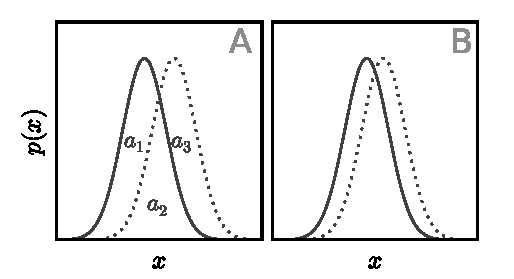
\includegraphics[scale=1.0]{figs/normal_example.pdf}
	\caption{
	  	Normal distributions exhibiting a total variational distance
		of (A) 50\% and (B) 30\%.  The total variational distance is 
		the non-overlapping portion of the distributions, e.g. in
		(A) it is given by 
		$\theta = a_1 / (a_1 + a_2) = a_3 / (a_2 + a_3)$.
	}
	\label{fig:l1_example}
\end{figure}

Empirically measuring the divergence between distributions
is a matter of ongoing
research \cite{val-thesis,batu2013testing,chan2014optimal}.
In the ``naive'' approach one first uses the samples to reconstruct 
empirical
distributions, by calculating their maximum likelihood parameters.
Then, one substitutes the empirical values of $p(x)$ and $q(x)$ into 
Equation~\ref{eq:theta} \cite{batu2013testing}.  
For example, one might directly estimate $\hat{p}(x) = N_x/N$, 
where $N_x$ is the number of times response $x$ is observed among $N$ 
total responses.

However this approach can \textit{drastically} overestimate $\theta$
\cite{val-thesis}.  As an illustrative example,
suppose that we have sampled two sets of 1000 words from \textit{possibly} 
different distributions, and that we wish to estimate the divergence 
between these distributions.  
It turns out that, if both sets of words were actually drawn from 
an identical Zipf distribution\footnote{The 
  Zipf distribution is a model for word frequencies 
  \cite{powers1998applications,zipf1949human}:
  \begin{align}
	p(x) = \frac{x^{-1}}{\sum_{n=1}^{\infty}x^{-1}},
	\label{eq:zipf}
  \end{align}
  where $p(x)$ is the probability of the $x$th most common word.
}, the naive approach would typically lead one to report 
$\hat{\theta} \approx 65\%$, even though, in reality $\theta = 0\%$
(this can be shown by simulated sampling).

Nevertheless, we can establish a lower bound for $\theta$ by 
exploiting a fact about the theoretical limits on the accuracy of a 
classifier algorithm.  The intuition is as follows: 
suppose workers are shown one of two alternative designs\footnote{We
use ``design'' in a general sense, to include both the design of the task
and of its context.  In particular, the ``design'' might include the
selection of tasks that were shown beforehand, or the use of framing.}
for an otherwise
similar task, and that we build a classifier which, 
based on a worker's response, infers which of the designs had been 
used.
If worker's responses are not affected by the design alternative,
then the classification problem will be hard, and the classifier's 
accuracy poor.
Conversely, if the classifier accuracy is good, then design alternative 
must have had a strong effect on the response distribution.

Stated formally, any classifier algorithm, $\mathcal{A}$, that
takes the response, $x$, of a worker, and guesses the 
design that elicited the response (from two possibilities:
$\mathrm{design}_1$ or $\mathrm{design}_2$), will do so with accuracy 
$\eta_\mathcal{A}$, that is bounded according to:
\begin{equation}
	\theta \geq 2\eta_\mathcal{A} - 1,
	\label{eq:sup:l1}
\end{equation}
where $\theta$ is the total variational distance between the 
distributions of responses
to $\mathrm{design}_1$ and $\mathrm{design}_2$.

\begin{figure*}
	\centering
	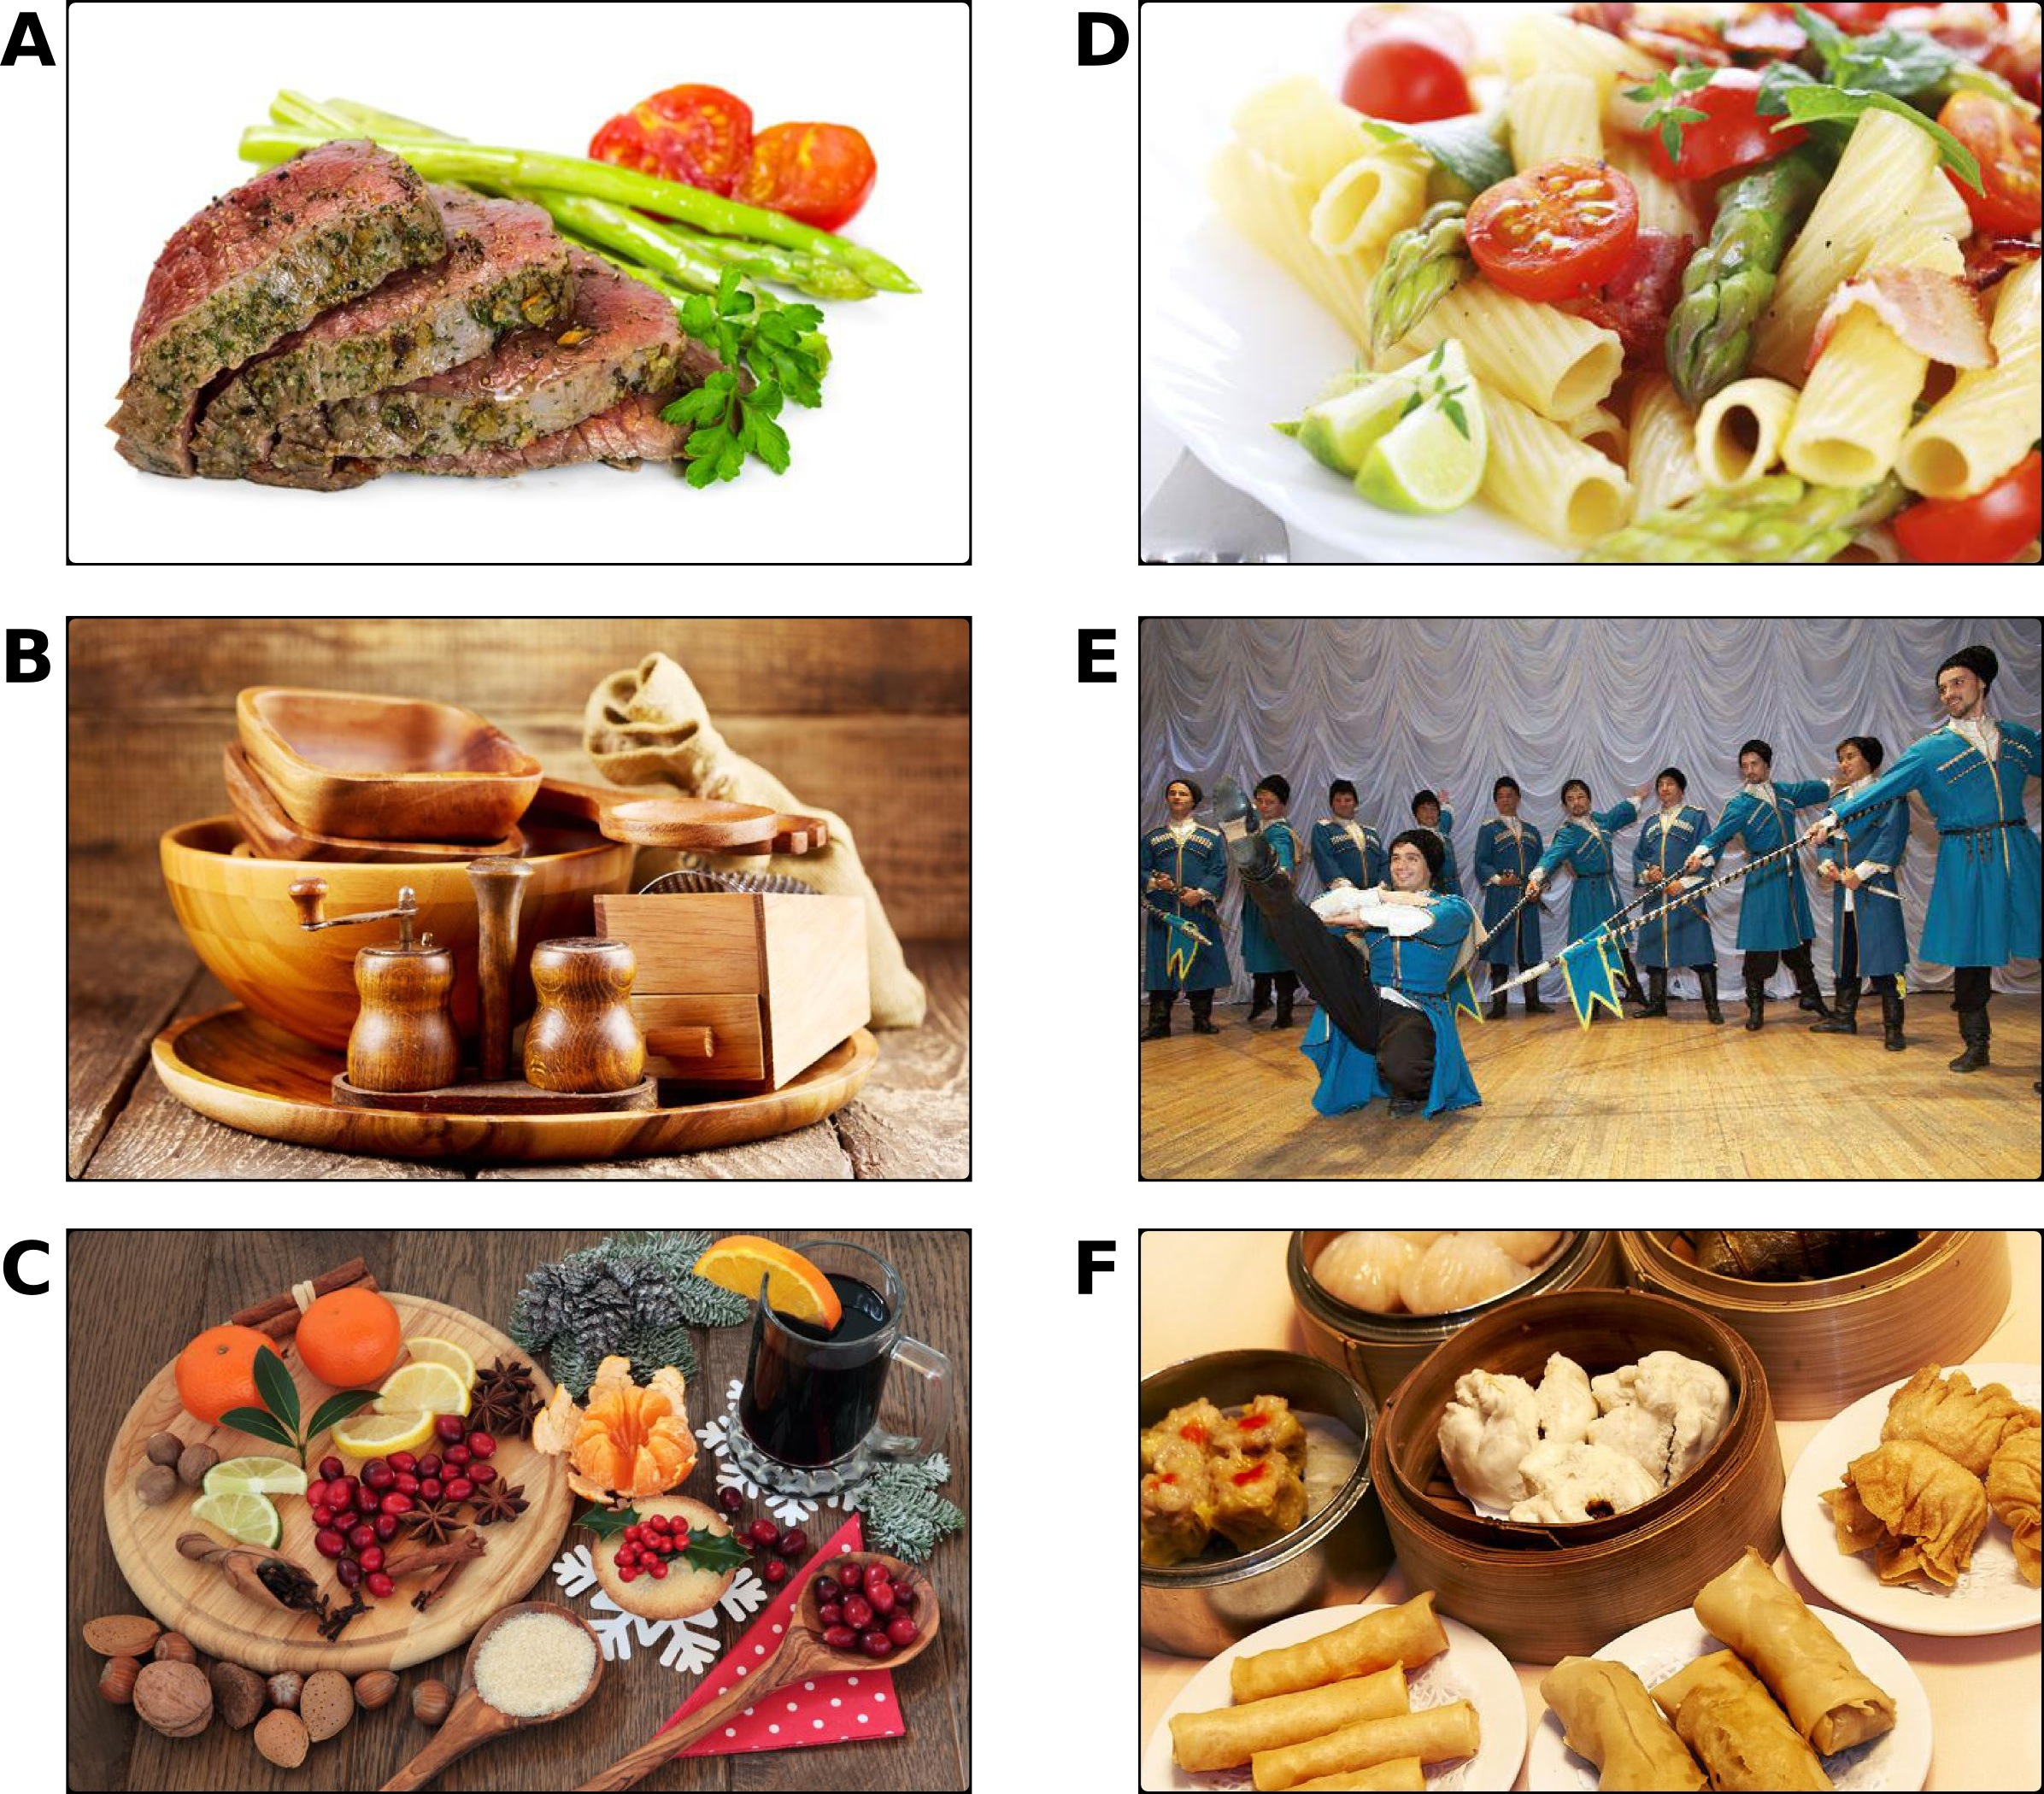
\includegraphics[scale=0.60]{figs/images.png}
	\caption{
		Examples of images used in
		initial tasks for the (\textbf{A}) \textit{food} and (\textbf{B}) 
		\textit{objects} treatments of \textit{intertask-food-objects};
		(\textbf{C}) test tasks for \textit{intertask-food-objects} and 
		\textit{frame-food-objects};
		initial tasks for the (\textbf{D}) \textit{food} and (\textbf{E}) 
		\textit{culture} treatments of \textit{intertask-food-culture};
		and (\textbf{F}) test tasks for \textit{intertask-food-culture} and 
		\textit{frame-food-culture}.
	}

	\label{fig:task}
\end{figure*}

We can establish Inequality~\ref{eq:sup:l1} by considering an
optimal classifier having accuracy $\eta_*$.  
Let us assume that workers are shown 
$\mathrm{design}_1$ or $\mathrm{design}_2$ with equal probability.
If the worker gives the response $x$, the optimal classifier must guess
that the worker was shown the design most likely to elicit $x$.
In other words, if $p_i(x)$ is the probability that a worker shown 
$\mathrm{design}_i$ responds with $x$, then it is optimal to 
guess that the worker saw $\mathrm{design}_j$, where 
$j = \arg\max_j{p_j(x)}$.

Of course, neither $p_1(x)$ nor $p_2(x)$ are known.  But, on seeing $x$,
the probability that such a classifier would be correct is:
\begin{align}
  \mathrm{Pr}\{\mathrm{correct}|x\} = \frac{1}{2} 
	+ \frac{|p_1(x) - p_2(x)|}{2(p_1(x) + p_2(x))}
\end{align}
Summing over all possible responses that a worker could provide, 
$x \in \mathcal{X}$, weighted by the probability of observing $x$, 
we obtain the accuracy of the optimal classifier:
\begin{align}
\eta_* 
  &= \sum_{x\in\mathcal{X}} 
	\mathrm{Pr}\{\mathrm{correct}|x\}\mathrm{Pr}\{x\} \\
  &= \sum_{x\in\mathcal{X}} 
	\left(
	\frac{1}{2} + \frac{|p_1(x) - p_2(x)|}{2(p_1(x) + p_2(x))}
  \right) \left( 
	\frac{p_1(x) + p_2(x)}{2} 
  \right) \\
  &= \frac{1 + \theta}{2}
\end{align}
Since no classifier can be more accurate than an optimal classifier,
it follows that, for any \textit{practical classifier} 
with accuracy $\eta_\mathcal{A}$, the bound 
$\theta \geq 2\eta_\mathcal{A} -1$ holds.

Thus, we can establish a \textit{lower bound} on $\theta$ by first 
building a classifier that infers the design shown to workers from their 
responses, and then measuring its accuracy.

\section{Experiment 1}
\subsection{Setup}
%\begin{figure}
%	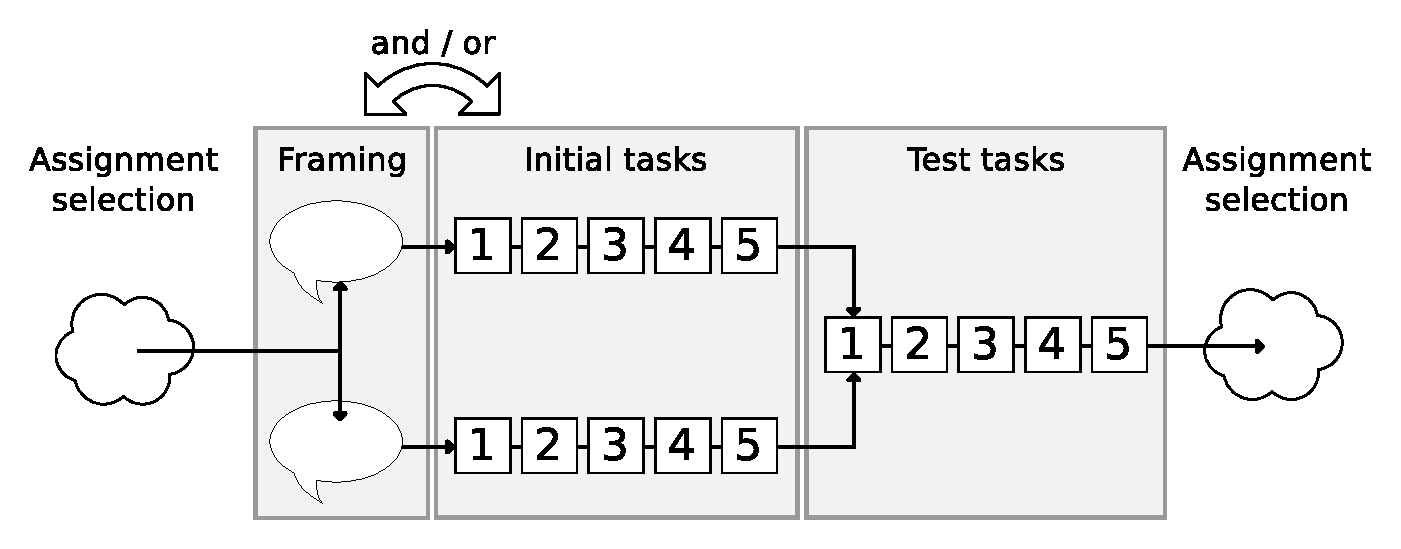
\includegraphics[scale=0.36]{figs/task-schematic-2.pdf}
%	\caption{
%	  Template for the experiments described in the main text.
%	  After selecting our assignment on Mechanical 
%	  Turk, workers were separated into two treatments.
%	  Workers from each treatment were subjected to framing and/or
%	  five initial tasks, which differed between treatments, and then 
%	  completed a set of five test tasks that were identical for both
%	  treatments.  Most experiments involved either framing or initial
%	  tasks (see table \ref{table:experiments}), 
%	  but \textit{frame-food-culture} involved both.
%	  After the experiment, workers return to the Mechanical Turk 
%	  task-selection interface.
%	}
%	\label{fig:task-schematic}
%\end{figure}

The first experiment we performed consisted of two sub-experiments which
we will call ``intertask'' and ``framing'', because they are respectively
designed to measure intertask and framing effects.  The experiment was 
performed on MTurk using 476 workers.  Workers
could only participate once in a given experiment, and could only 
participate in one of the experiments we present here.  Workers were 
required to have had 90\% of their previously submitted work on Mturk 
accepted by other requesters to participate.  No other screening 
was applied to workers.

The experiment was conducted using a single HIT\footnote{
  On MTurk, a HIT (or Human Intelligence Task) is the smallest 
  assignable unit of work.  The use of ``Task'' in HIT differs from that
  used here; here labeling a single image is considered to be one ``task'',
  and so a HIT is actually composed of 10 tasks.
}.  Workers who accepted the HIT were randomly assigned to one of the two
sub-experiments.  Both sub-experiments consisted of two treatments, which
we call ``food'' and ``culture'', and workers were also randomly 
assigned to a treatment, resulting in 119 workers per treatment.  
In both treatments of both sub-experiments,
workers were asked to perform ten image-labeling tasks, each of which 
required the worker to assign five descriptive labels to an image.  
Labels had to contain at least two letters to be accepted. 
Workers were paid USD\$0.45 for their work.
In all cases, the last five tasks were identical among all treatments 
(and across sub-experiments), and were presented in the same order.  
These last five tasks constituted the ``test tasks'', whose distribution
of responses could admit intertask or framing effects.

In the intertask sub-experiment, we varied the first five tasks given to 
workers based on the treatment.  Workers assigned to the ``food'' 
treatment were shown images of food (see Figure~\ref{fig:task}A), 
while workers assigned to the ``culture'' treatment were shown other kinds 
of cultural depictions, such as dance, sport, and 
music\footnote{
  We do not assert that cultural practices can be cleanly separated into 
  food-related and non-food related ones, nor is a strict division 
  necessary for our analysis.
} (see Figure~\ref{fig:task}B).  
However, within a given treatment, workers were shown the same images in
the same order.  As mentioned, workers 
from both treatments then performed the same five test tasks.  The test
tasks consisted of images depicting meals of diverse ethnic origin
(see Figure~\ref{fig:task}C).
From the perspective of the worker, there was no distinction between the 
initial and test tasks.

In the framing sub-experiment, we did not vary the initial tasks, but 
instead, introduced a \textit{framing slide} before the tasks.  
Depending on the treatment, the framing slide read 
``This research is proudly funded by The National Foundation for 
Nutritional Awareness'', or ``\ldots by the Global Foundation for the 
Recognition of Cultures''.  The intention was to frame the task by
providing the name of a (fictitious) funder, while using names that
invite the worker to focus on different aspects of the image content.  
Initial tasks were still included to ensure that learning or fatigue 
effects were equalized between the sub-experiments.  
For the initial tasks, we used the same images as had been shown to the 
food treatment of the intertask sub-experiment.  
If intertask effects exist, any choice of images for the initial tasks 
will have an effect.  This choice makes the food treatments of both 
sub-experiments very similar, so that the culture treatments of both 
sub-experiments can be viewed as perturbations from a similar baseline.  
The test tasks were the same as for the intertask sub-experiment.

Manual inspection showed that the vast majority of labels were of 
high-quality.  Less than 1\% of submissions were problematic, having
redundant labels or entries that were not English words.
We chose to include all submissions for analysis in the experiments
presented here.

\subsection{Results}

\begin{figure}[t]
    \centering
	\includegraphics[scale=0.85]{figs/theta-exp1.pdf}
	\caption{
	    Lower bound total variational distance ($\theta_\mathrm{NB}$) 
		between responses given
		by workers on test tasks in Experiment 1, when they have been 
		shown different initial tasks (intertask), or been exposed to
		different framing (framing), as determined using naive Bayes 
		classifiers.  Standard error bars are shown.
	}
	\label{fig:theta-exp1}
\end{figure}

\paragraph{Existence of intertask and framing effects.} 
Looking at the frequencies with which workers used words, we tested for
heterogeneity between the two treatments of each sub-experiment.
For the intertask sub-experiment, we found the responses 
for the two treatments differed significantly 
(by $\chi^2$ test, $p<0.001$), 
demonstrating that intertask effects do exist.  However, we did not find 
significant effects due to framing ($p=0.29$).

Testing for heterogeneity of word-frequencies was based on 
Pearson's $\chi^2$ test with Yates' correction.
In linguistics applications, the use of a $\chi^2$ to test for 
heterogeneity between corpora has been called
into question, because there is frequently heterogeneity \textit{within}
a given corpus \cite{kilgarriff1996comparing}.
This occurs because certain documents in a corpus will regard certain 
topics, leading to bursty word usage.  While our setup is substantially
remote from the applications for which this concern was raised, 
one could argue that the responses to a given treatment
constitute a ``corpus'', and the responses of a given worker to a 
``document''.
To address this concern, we randomly split responses to given treatment
into two sets, and tested for heterogeneity between the sets.
In all cases, we failed to find heterogeneity \textit{within} a given 
treatment (with $p > 0.3$ for all treatments and $p > 0.8$ for most).
These results hold for Experiment 2, to be discussed later.
Thus, the heterogeneity we observed \textit{between} the intertask 
treatments indicates a meaningful effect.

\pagebreak
\paragraph{Strength of intertask and framing effects.}
Having affirmed the \textit{existence} of intertask effects, we sought to
measure their strength, i.e. $\theta$.
To measure $\theta$ we created a naive Bayes classifier based on a 
multinomial distribution over the word frequencies in worker's labels, 
and measured it's accuracy using leave-one-out cross-validation.  
We chose the naive Bayes
classifier for three reasons.  First, it performs well even when the 
number of features is large compared to the number of training examples
\cite{bickel2004,hastie2009elements}.  
Second, there are no hyperparameters to 
optimize, which eliminates the need to partition the response data into
dev and test sets.
Third, the conditional independence assumption, normally 
undertaken for pragmatic reasons \cite{Zhang2004562}, 
is probably mild in 
relation to image labels, since they are likely to be less dependent
on one another than in a coherent passage of text.  We repeated our
analysis using support vector machines and found very similar results.

To produce word frequency features, worker-submitted labels were split on 
white
space and punctuation, and the resulting tokens were spell-corrected based
on edit-distance to a dictionary of words, followed by stop-word removal
and lemmatization.  The spelling correction
dictionary was compiled from a combination of WordNet 
\cite{felbaum1998wordnet} and words
collected by crawling the World Food section of \url{allrecipes.com}.

Based on the performance of the classifier, intertask effects altered
workers' responses, leading to (a lower bound of) 51.3\% total variational 
distance in their response distributions (Figure~\ref{fig:theta-exp1}).  
This represents a remarkably strong effect.
Visually comparing two word frequency distributions is difficult, but 
Figure~\ref{fig:l1_example} provides an example of distributions having 
$\theta = 50\%$.  In contrast, the effect due to framing, was not 
significantly different from zero (Figure~\ref{fig:theta-exp1}).
And so, intertask effects were stronger than the effects due to 
framing ($p<0.001$)\footnote{
  To compare framing and intertask 
  effects, we approximated the distribution
  of correct classifications as a normal distribution, and performed
  a (two-tailed) two-proportion $z$-test.
}.
In other words, the \textit{microtasks themselves} had a stronger effect 
than framing.

When observing the classifier's accuracy, in order to calculate $\theta$,
the number of correct inferences made by the classifier follows a binomial 
distribution.  The fraction of successes yields the maximum likelihood
estimate of the classifier's accuracy (used to generate $\theta$), 
and we derived confidence intervals using the exact Clopper-Pearson method.

The results from the first experiment clearly show that intertask effects 
arise and are strong.  On the other hand, we were scarcely able to observe
any effect due to framing.  This raises a few questions which we seek
to answer using a second experiment.  The first question is simply whether
the result will replicate using different sets of images.  
If so, then as the next question, we may ask how intertask effects evolve
as the worker performs tasks.  Presumably, intertask effects wear off at 
some point, but is it after one task, two, or more?  

Using the results from Experiment 1, 
we could look at the intertask effects for individual test questions, 
however, each question uses a distinct image, whose own content may
modulate the extent to which it can be influenced by intertask effects.
We cannot disentangle the effects of task position from that of image 
content in Experiment 1.

In setting up Experiment 2, we also wish to increase the strength of 
framing.  While it was remarkable that intertask effects were stronger 
than the framing effects elicited in the first experiment, perhaps the 
most meaningful comparison is one which shows just how extreme framing 
treatments need to be to produce effects on par with intertask effects.  
One factor that may have weakened the effects of framing in Experiment 1 
is the inclusion of initial tasks between the framing slide and the test 
tasks. They were included to ensure that workers had always completed the
same number of tasks before beginning the test tasks.  However, their 
inclusion gives time for differential framing effects to 
subside, while also generating intertask effects that are 
\textit{shared} between the treatments, potentially masking the framing 
effects that remain.  In the next experiment, we measure framing effects 
immediately after the application of framing.

\section{Experiment 2}
\subsection{Setup}
In Experiment 2 we again had ``intertask'' and ``framing'' 
sub-experiments, but we included a third sub-experiment, ``echo'', which 
incorporated more extreme framing treatments.  
As before, each sub-experiment had
two treatments, but this time they were ``food'' and ``objects''.
Keeping a food treatment enabled us to perform deeper lexical analysis of 
both experiments (to be discussed in the results for Experiment 2).  
The experiment was again performed using a single HIT on MTurk, 
and involved 1666 workers.
Workers were randomly assigned to a sub-experiment and treatment upon
starting the HIT, resulting in 119 workers per treatment.

The intertask sub-experiment was similar to that in Experiment 1: workers
performed a set of five initial tasks, whose images depended on the 
treatment to which they had been assigned, and then performed the test 
tasks, which were common to both intertask treatments (as well as to both 
treatments of the other sub-experiments in Experiment 2).  
In the food treatment, 
the initial tasks contained images of food (see Figure~\ref{fig:task}D).  
This time, care was taken to exclude any non-food items, 
such as utensils or place-settings, except, in some cases, for the plate
supporting the food itself.  In the objects treatment, initial tasks 
contained images depicting table settings and various non-food objects one 
might find in a kitchen, but no food (see Figure~\ref{fig:task}E).  
The images in the test tasks,
depicted both food and non-food objects together 
(see Figure~\ref{fig:task}F).

In contrast to Experiment 1, we performed five replicates of the intertask
sub-experiment, each time permuting the test tasks.  The test tasks were
``rotated'' in such a way that, what was the first test task became
the second, the second became the third, and so on up until the last test
task, which became the first.  In this way, each of the five positions
was occupied by each test task, enabling us to disentangle the effect of
test task position (relative to initial tasks) from test task content,
and thereby see how intertask effects vary as a function of position in
the task sequence.

The framing sub-experiment was similar to that from Experiment 1, except
that we omitted initial tasks altogether, so that the test tasks followed
immediately after framing.  This meant that workers would not have 
performed any tasks by the time they began the test tasks.  While that will
hold constant for both framing treatments, and thus not produce a 
differential effect, the workers may be more (or less) susceptible to 
influences during their first few tasks.  One can expect framing effects
to be stronger than in Experiment 1, because of the immediacy with which
the test tasks follow the framing.  The framing slide for the food 
treatment read ``Funded by the laboratory for the visual perception of 
Food and Ingredients'', and for the objects treatment it read ``\ldots
perception of Objects and Tools''.

We introduced the echo sub-experiment to produce the strongest framing 
effects.  This sub-experiment was similar to the framing sub-experiment,
but differed in two ways.  First, the framing slide stated an explicit
purpose for the study: ``The purpose of this study is to understand the 
visual perception of Food and Ingredients'' 
and ``\ldots of Objects and Tools''.  Second, before moving past the
framing slide, workers were asked what the purpose of the study was, and
had to respond by selecting the framing statement from among a short
list in a combo-box.  It is because workers had to echo the framing 
statement using a combo-box that we call this sub-experiment ``echo''.

\subsection{Results}

\begin{figure}[t]
    \centering
	\includegraphics[scale=0.85]{figs/theta-exp2.pdf}
	\caption{
	    (\textbf{A}) Lower bound total variational distance 
		($\theta_\mathrm{NB}$), between 
		responses given to test tasks in experiment 2 
		when workers were shown different initial tasks (intertask), 
		or were exposed to different framing treatments (framing), or 
		echoed framing treatments (echo).
		(\textbf{B}) Detail of the effects seen from showing
		workers different initial tasks (corresponding to intertask in 
		panel A), now broken out for each of the five test task positions.
		As workers proceeded through test tasks, intertask effects waned
		but remained significant ($p<0.05$) even for the fifth test task.
		Standard error bars are shown.
	}
	\label{fig:theta}
\end{figure}

%\begin{table}[b!]
%\small
%\centering
%\setlength{\tabcolsep}{1pt}
%\begin{tabular}{c c c c c}
%\toprule
%Experiment & \parbox[c]{3.0cm}{\centering{Priming modality}} & Initial Tasks & Frame \\
%\midrule
%\multirow{2}{*}{\textit{intertask-food-objects}} 
%& \multirow{2}{*}{initial tasks} & \textit{food} & none \\
%  & & \textit{objects} & none  \\
%
%\noalign{\smallskip}
%\hdashline
%\noalign{\smallskip}
%
%\multirow{2}{*}{\textit{frame-food-objects}} 
%& \multirow{2}{*}{framing} & none 
%	& ``food''\textsuperscript{a} \\
%& & none 
%	& ``objects''\textsuperscript{b} \\
%
%\noalign{\smallskip}
%\hdashline
%\noalign{\smallskip}
%
%\multirow{2}{*}{\textit{echo-food-objects}} 
%& \multirow{2}{*}{echoed framing} & none
%	& ``food''\textsuperscript{c} \\
%& & none & ``objects''\textsuperscript{d} \\
%
%\noalign{\smallskip}
%\hdashline
%\noalign{\smallskip}
%
%\multirow{2}{*}{\textit{intertask-food-culture}} 
%& \multirow{2}{*}{initial tasks} & \textit{food} 
%	& none \\
%& & \textit{culture} 
%	& none \\
%
%\noalign{\smallskip}
%\hdashline
%\noalign{\smallskip}
%
%\multirow{2}{*}{\textit{frame-food-culture}} 
%& \multirow{2}{*}{framing} & \textit{food} 
%	& ``food''\textsuperscript{e} \\
%  & & \textit{food}
%	& ``culture''\textsuperscript{f} \\
%
%\bottomrule
%\end{tabular}
%\caption{
%	Description of experiments performed.  Each experiment had two treatments
%	which differed either in the initial tasks shown or the framing used 
%	(the priming modality).  
%	During echoed framing, the worker had to respond to the framing language
%	using a combo box input.  The framing language used was as follows:
%	\newline\textsuperscript{a} ``Funded by the laboratory for the visual 
%		perception of Food and Ingredients''
%	\newline\textsuperscript{b} ``Funded by the laboratory for the visual 
%		perception of Objects and Tools''
%	\newline\textsuperscript{c} ``The purpose of this study is to understand the visual perception of Food and Ingredients''
%	\newline\textsuperscript{d} ``The purpose of this study is to understand the visual perception of Objects and Tools''
%	\newline\textsuperscript{e} ``This research is proudly funded by The National 
%		Foundation for Nutritional Awareness''
%	\newline\textsuperscript{f} ``This research is proudly funded by The Global 
%		Foundation for the Recognition of Cultures''
%}
%\label{table:experiments}
%\end{table}

\paragraph{Existence and strength of effects.}
As in the previous experiment, intertask effects led to significant 
changes in the words workers used to label images in the intertask 
sub-experiment ($p<0.001$).  Based on
the performance of a naive Bayes classifier, the strength of the effect 
was (as a lower bound) $\theta=30.6\%$ total variational distance
(see Figure~\ref{fig:theta}A).  Again, it is difficult to visualize the 
distributions of word frequencies, but for reference, the distributions 
shown in Figure~\ref{fig:l1_example}B have $\theta = 30\%$.  

This time, the framing sub-experiment also showed a significant effect.
Framing induced changes in the frequencies of word usage at significance 
(as determined by $\chi^2$ test; $p=0.0012$).  However, 
the \textit{extent} of the effect could not be distinguished from zero
($p =0.37$) based on the performance of a naive Bayes classifier 
(Figure~\ref{fig:theta}A).
As in Experiment 1, we found that intertask effects were stronger than
framing effects ($p<0.001$).

It was only in the echo sub-experiment that framing effects were on par 
with intertask effects.  In this sub-experiment, framing influenced 
workers responses ($p<0.001$), and the performance of a naive 
Bayes classifier showed that it produced (lower bound) 36.1\% total 
variational distance in worker responses (Figure~\ref{fig:theta}A).  The
strength of effects due to echoed framing could not be distinguished
from that of intertask effects ($p=0.79$).

It is remarkable that intertask effects were on par with an explicit, 
actively reinforced statement of the tasks' purpose.
Requiring the worker to reiterate the purpose signals our intent, as the 
requester, to ensure that the worker has taken note of it, 
possibly leading the worker to interpret the exchange as an instruction.  

\paragraph{Persistence of intertask effects.} 
Taking advantage of the replicated intertask sub-experiment, we created
a naive Bayes classifier for each test task, when it occurs at each test 
task position.  
Thus, for each of the five test task positions, we obtained 
five separate measures of the intertask effect strength (one for each of 
the test tasks, when occupying that position).  We averaged these five 
measurements to produce the intertask effect strength for the given task
position, and these values are shown in Figure~\ref{fig:theta}B.

Not surprisingly, the first test task shows the strongest intertask 
effects, at 28.1\% total variational distance.  The effect appears to 
drop suddenly after the first test task, but remain significant 
right through until the fifth task position ($p=0.030$).
Remarkably, even after four intervening tasks, the effect of 
having performed different initial tasks shifts worker's responses to the
fifth test task by 12.4\% total variational distance.

\begin{figure}
	\centering
	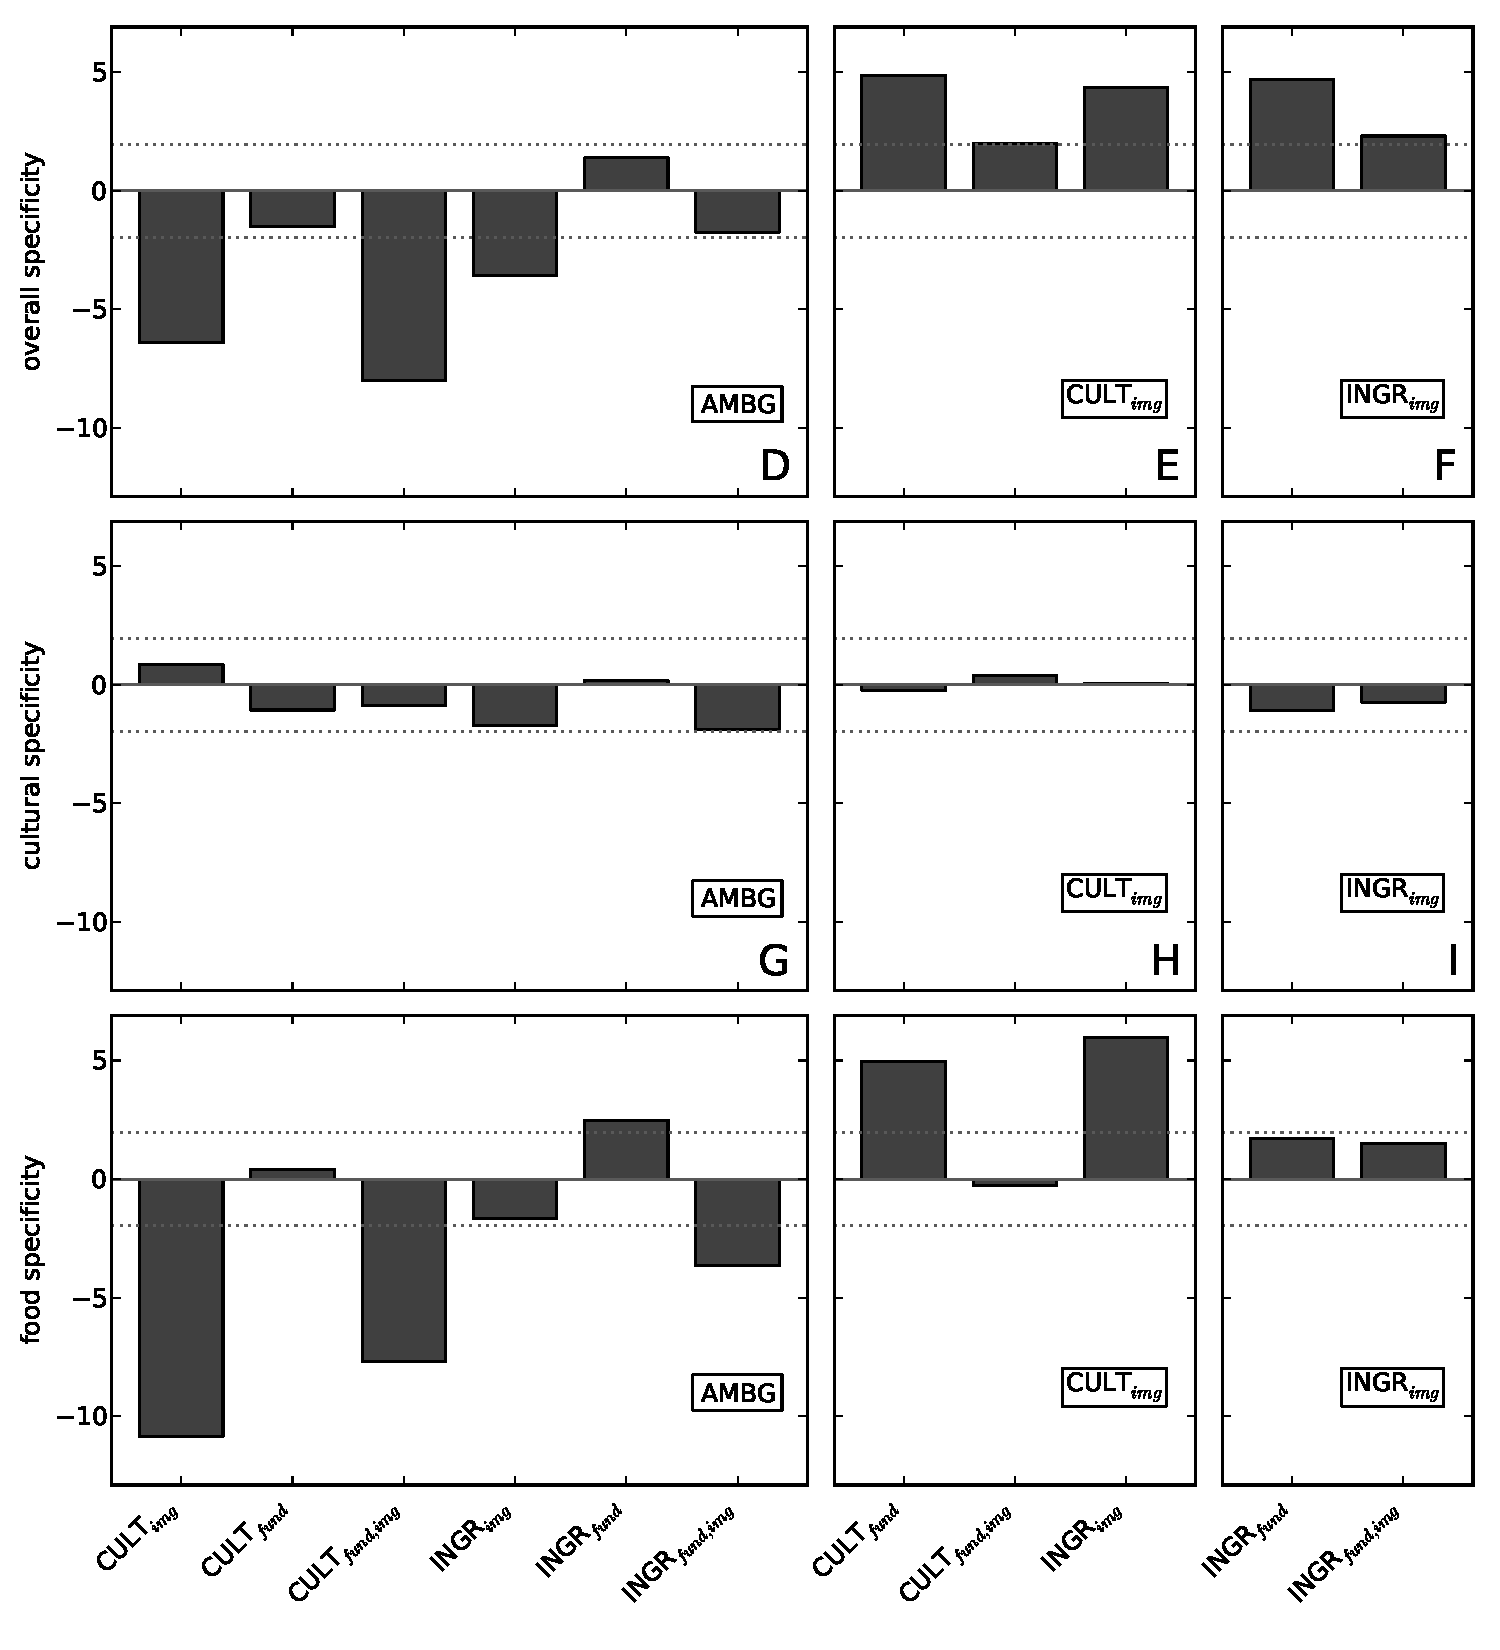
\includegraphics[scale=0.97]{figs/specificity.pdf}
	\caption{
		Workers exposed to food (either in framing or initial tasks)
		showed a different tendency to focus on food when labeling
		test tasks, and their vocabulary in reference to food was affected.
		In all three plots, positive values indicate a larger quantity for 
		workers from the food treatment.
		(\textbf{A}) Exposing workers to food significantly changed the 
		fraction of food references they provide, but did not necessarily 
		\textit{increase} it.
		(\textbf{B}) The number of unique food-related
		words (richness) was greater for food-exposed workers, 
		except in the 
		case of the framing sub-experiment of Experiment 1 
		(stars indicate the threshold
		for a significant deviation, $\alpha=0.05$). 
		(\textbf{C}) Food-exposed
		workers used more specialized words to refer to food.
		Standard error bars are shown in (\textbf{A}) and (\textbf{C}).
	}
	\label{fig:specificity}
\end{figure}

\begin{table*}
	\centering
	\setlength{\tabcolsep}{4pt}
	\begin{tabular}{ c c c c c }
	

		\setlength{\tabcolsep}{4pt}
		\begin{tabular}{ r | c }
		\toprule
		\multicolumn{2}{c}{
			\parbox[c]{2.5cm}{
				\centering
			Exp. 1 intertask} 
		}\\
		\midrule
		spicy & 26 \\
		sauce & 17 \\
		indian & 15 \\
		buffet & 14 \\
		exotic & 12 \\
		festival & -11 \\
		offering & -12 \\
		statue & -15 \\
		india & -20 \\
		food & -56 \\
		\bottomrule
		\end{tabular}

&

		\setlength{\tabcolsep}{4pt}
		\begin{tabular}{ r | c }
		\toprule
		\multicolumn{2}{c}{
			\parbox[c]{2.5cm}{
				\centering
			Exp. 1 framing} 
		}\\
		\noalign{\smallskip}
		\midrule
		indian & 11 \\
		banquet & 8 \\
		spicy & 7 \\
		asian & 6 \\
		variety & 6 \\
		delicious & -6 \\
		meat & -7 \\
		festival & -7 \\
		spice & -7 \\
		food & -9 \\
		\bottomrule
		\end{tabular}

&

		\setlength{\tabcolsep}{4pt}
		\begin{tabular}{ r | c }
		\toprule
		\multicolumn{2}{c}{
			\parbox[c]{2.5cm}{
				\centering
					Exp. 2 intertask
			}} \\
		\midrule
		coffee & 38 \\
		meal & 34 \\
		cheese & 34 \\
		apple & 32 \\
		dessert & 21 \\
		cup & -30 \\
		glass & -45 \\
		table & -70 \\
		candle & -74 \\
		food & -80 \\
		\bottomrule
		\end{tabular}

&

		\setlength{\tabcolsep}{4pt}
		\begin{tabular}{ r | c }
		\toprule
		\multicolumn{2}{c}{
			\parbox[c]{2.5cm}{
				\centering
				Exp. 2 framing
			}
		}\\
		\midrule
		bread & 18 \\
		wine & 18 \\
		cheese & 16 \\
		apple & 14 \\
		oil & 12 \\
		table & -9 \\
		meal & -10 \\
		candle & -12 \\
		dinner & -13 \\
		food & -32 \\
		\bottomrule
		\end{tabular}

&

		\setlength{\tabcolsep}{4pt}
		\begin{tabular}{ r | c }
		\toprule
		\multicolumn{2}{c}{
			\parbox[c]{2.5cm}{
				\centering
			Exp. 2 echo } 
		}\\
		\midrule
		apple & 24 \\
		cheese & 23 \\
		wine & 15 \\
		coffee & 14 \\
		oil & 7 \\
		knife & -24 \\
		dinner & -26 \\
		fork & -27 \\
		candle & -35 \\
		food & -55 \\
		\bottomrule
		\end{tabular}


	\end{tabular}
	\caption{
		The five words whose frequencies as labels for the first test
		task increased (or decreased) the most between treatments of the
		given sub-experiments.
		Values indicate the absolute change in number of occurrences
		of the word, and positive values indicate that the food-exposed
		treatment 
		used the word with higher frequency.  
		Note that the word ``food'' is always the most suppressed among
		food-exposed workers.
	}
	\label{table:top-words}
\end{table*}

\paragraph{Intertask effects and concept activation.} 
To gain further insight into the nature of intertask effects, 
we investigated the vocabulary that workers used to label test tasks. 
One might expect that, within a given experiment, those workers exposed 
to food (whether through framing or initial
tasks) would label test tasks using 
food-related words more often.  To test this we developed an 
automated approach to labeling food-words based on the 
WordNet knowledge base \cite{felbaum1998wordnet}.  

WordNet provides
hyponym and hypernym relations between words.  A hypernym is a 
generalization (for example, ``bread'' is a hypernym of ``pumpernickel''), 
while a hyponym is a specialization.  We took the set of food-words
to be all those reachable through
a chain of hyponym relations from the word-senses 
\texttt{food.n.01} and \texttt{food.n.02}, in other words, all words
denoting a specific kind of food (a total of 3590 words).  
To improve the coverage of words for
less common foods, we augmented this set with all words
discovered while crawling the World Food section of \url{allrecipes.com} 
which were not already in WordNet.  

To validate the resulting set of 
food words, three independent annotators labeled 500 words selected from 
workers' responses as either food or non-food, and these were
compared to the labels derived using the automated approach.
Among those words, 26\% were 
deemed to be food by the majority of annotators.  
Taking the majority label among annotators to be the correct one, 
the automatically-identified food-words
had 88\% correspondence to the human annotators.  Treating the
automated identification of food words as another annotator, there 
was an 82.4\% agreement between annotators.

Using the automated labeling of food words, we found that, contrary to
expectations,
workers exposed to food (via prior tasks or framing) did not necessarily
use more food-words when labeling images in the test tasks.
In the intertask treatment of Experiment 1, workers from the food treatment
actually used significantly\footnote{
  Frequencies of food references within a treatment were calculated as
  an average across workers, and modeled as normally distributed.
} \textit{fewer} food-related words 
during test tasks (Figure~\ref{fig:specificity}A).  This finding
rules out a seemingly-simple idea that workers emphasize
content seen in earlier tasks.  Seeing given content significantly 
influences workers' propensity to refer to it in subsequent tasks, but it 
does not necessarily \textit{increase} it.

To deepen our understanding, we investigated workers' lexical richness in 
reference to food, that is, the number of \textit{unique} food-related 
words used.  Even if workers provide an abundance of food-related words, 
there can be less diversity, if, for example, workers repeat generic 
references to food.
The \textit{intertask} sub-experiments from both Experiments 1 and 2 showed
that workers from the food treatments had
greater lexical richness, in reference to food, than their counterparts 
(as much as 20\% more) (Figure~\ref{fig:specificity}B).  
This is particularly noteworthy for the intertask sub-experiment in 
Experiment 1, because there,
workers from the food treatment made fewer total references to food.  
Thus, although prior task exposure does not necessarily increase the 
propensity
to identify content in later tasks, it does appear to activate vocabulary 
pertaining to content in the prior tasks.

To test the significance of the difference in sizes of food
lexicons,
we created a null model for each experiment, by assuming that
responses for both treatments were in fact drawn from the same 
distribution.
This was accomplished by pooling responses for both treatments 
of a given experiment, then 
drawing two bootstrap samples of 119 responses and calculating
the difference in the size of their food lexicons.  
We repeated this 1000 times and took the 2.5th and 97.5th percentiles 
as the critical values for the rejection of the null hypothesis 
(the latter shown by stars in Figure~\ref{fig:specificity}B).

The above observations regarding lexical richness suggest that initial 
tasks might influence workers to use more \textit{refined} or 
\textit{specialized} words, when referring to aspects 
of content that had been present in the initial tasks.  
To test this directly, we used the hypernym and hyponym relations in 
WordNet to operationalize the notion of word specialization.  
Within each sub-experiment, we determined the relative specificity
of the food-words, between the treatments using the following equation:
\begin{equation}
	S(P,Q) = \frac{
		\sum_{w\in P}\sum_{v\in Q} \left(
			\mathbf{1}_{[w>v]} - \mathbf{1}_{[v>w]} \right)
	}{
		\sum_{w\in P}\sum_{v\in Q} \left(
			\mathbf{1}_{[w>v]} + \mathbf{1}_{[v>w]} \right)
	},
\end{equation}
where $P$ and $Q$ are sets of words associated to different experimental 
treatments, and $\mathbf{1}_{[w>v]}$ evaluates
to 1 if word $w$ is more specific than (i.e. is a hyponym of) word $v$.
The relative specificity lies within $[-1,1]$; 
we report it as a signed percentage.
In computing this quantity between two treatments, we first computed the 
relative specificity for the treatments separately for each test task, and 
averaged the results obtained across the five test tasks.  To establish
significance, we again used a null model, based on bootstrapping.

In all sub-experiments,
workers from the food treatment used more specialized words, 
in reference to food 
(about 15\% more; $p < 0.05$) (Figure~\ref{fig:specificity}C).
Except in the case of the framing treatment of Experiment 1, these 
between-treatment differences in word specialization were significant 
($p<0.05$).

It is interesting that such substantial increases in both the lexical 
richness and specialization of food-related words 
held for the intertask sub-experiment of Experiment 1, where, as mentioned,
we observed 
that food-exposed workers made \textit{fewer} references to food overall. 
These observations point 
to countervailing factors: one factor tending to activate the more 
specialized and less common food-related words 
(yielding greater lexical richness and specialization), and the other tending 
to suppress certain, presumably more common and generic words 
(yielding fewer food-related words in total).

This hypothesis is corroborated when we look at those words whose 
frequencies changed the most from one treatment to another 
(Table~\ref{table:top-words}).  
The word ``food'', which is the most generic possible food-related word, 
was always \textit{suppressed} among food-exposed workers, along with other
very generic food references being suppressed too, such as ``meal'' and 
``dinner''.  In fact, 
for all experiments, ``food'' was the \textit{most suppressed} word.
Meanwhile, the most activated food-related words, among food-exposed 
workers, tended to refer to specific foods, 
like ``apple'', ``cheese'', and ``bread''.

\section{Discussion}
Our results show that intertask effects exist, are very strong, and are
on par with the effect of an explicit statement of a task's purpose 
reinforced by requiring the worker to repeat that purpose.  
This very surprising 
result immediately raises follow-on questions for future work: 
what are the psychological mechanisms at play? How are other kinds of 
tasks (i.e. other than image 
labeling) impacted by intertask effects?  How can intertask effects best 
be used to produce optimal task design?  We expect these questions will
be fruitfully explored in future work.

While our setup does not allow us to tell what psychological mechanism(s) 
are responsible for intertask effects, we suspect that priming is involved.
As mentioned, we believe microtasks create conditions conducive to priming,
and this is what first lead us to suspect intertask effects might exist.  
Priming occurs when a prior stimulus causes a person to respond to a 
subsequent task with increased speed or 
accuracy, or with the ability to recognize briefer or 
noisier stimuli \cite{BJOP1796,BJOP1826,Huber2008324}.
In the case of image labeling, pre-activation of 
vocabulary relating to prior tasks, through a priming mechanism, 
could lead to more rapid retrieval of those words in subsequent tasks.  
A worker may be more likely to enter those words which enter her mind 
first, so priming could lead to certain words being preferred.  
As the worker
completes many tasks with a common theme, the worker's vocabulary relating
to that theme will be increasingly activated, enabling more specialized
words to be retrieved quickly, and therefore to be submitted as responses.

However, as we alluded to above, there appears to be countervailing 
factors:
while richness and specialization of food-related words always increased 
(or were not significantly changed) among workers exposed to food in 
initial tasks, the total number of references to food significantly 
\textit{decreased} in one case.  
Here we suspect \textit{negative} priming to be at play.
Negative priming occurs when, after exposure to a stimulus 
considered to be non-salient, subsequent recognition of the stimulus is 
inhibited \cite{mayr2007negative}.  In the case of our image labeling 
tasks, repeated exposure to images depicting food might cause the worker to
stop regarding the basic presence of food as salient, and to direct her 
attention instead to the features that are specific to the food in a given 
image.  This would explain the suppression of very generic references to 
food observed in Table~\ref{table:top-words}.  
The balance between the inhibition of generic food-related words, and the 
activation of specialized ones, could lead to more or less food references
overall, so this dual priming mechanism is consistent with our 
observations.  Direct experimentation is needed to determine whether
priming mechanisms, positive or negative, can explain intertask
effects.

Prior to this study, it was not realized that earlier microtasks could 
have such strong effects on later ones.
But our findings show this is an important design factor that 
should be considered by anyone using microtask platforms.
The commonly employed practice of randomizing task ordering probably
introduces a significant amount of noise due to intertask effects:
even chains of two or three similar tasks, which will not be reliably 
eliminated in random permutations, could lead to the levels of influence 
we observed in our experiments.  Preferably, a deeper understanding of 
intertask effects might allow them to be properly controlled.

But perhaps more importantly, our findings show that intertask effects 
might be leveraged obtain greater quality and reproducibility in 
crowdsourcing.
A consistent goal in human computation is the elicitation of expert-level
judgments from non-expert workers \cite{kittur2011crowdforge}.  
This has been achieved in some
applications \cite{snow2008cheap,Mortensen20131020,Warby2014385}. 
The distinction between experts and novices is partly attributable
to specialized knowledge and heuristics. 
But experts also simplify tasks by more efficiently directing 
their focus toward salient features \cite{kellman2009perceptual}.  
Using strategic task exposure during training, it might be possible to 
guide workers' focus and salience attribution, enabling expert-level 
judgment in a wider variety of crowdsourced applications.

Intertask effects are a new basic discovery in the quest to design 
reliable and reproducible tasks for human computation.
We anticipate future work will yield techniques to control intertask 
effects, to reduce unwanted bias, and to tune the focus, diversity, and 
specificity of worker responses.

\bibliographystyle{SIGCHI-Reference-Format}
\bibliography{newbib}

\end{document}

%%% Local Variables:
%%% mode: latex
%%% TeX-master: t
%%% End:
